\documentclass[12pt,a4paper]{report}
\usepackage[utf8]{inputenc}
\usepackage[T1]{fontenc}
\usepackage[french]{babel}
\usepackage[french]{nomencl}
\usepackage{lmodern}
\usepackage{graphicx} %Pour les images 
\usepackage{amsmath}
\usepackage{amsfonts}
\usepackage{amssymb}
\usepackage{makeidx}
\usepackage{array} %pour les tableaux \centering pour centrer le tout dans page.
\usepackage{tabularx} %gère automatiqueent la taille du tableau
\usepackage[left=2cm,right=2cm,top=2.5cm,bottom=2.5cm]{geometry}

%Interligne 1.5
\renewcommand{\baselinestretch}{1.5}

%Pour la page de garde
\newcommand{\hsp}{\hspace{20pt}}
\newcommand{\HRule}{\rule{\linewidth}{0.5mm}}

%HyperRef Conf
\usepackage{hyperref}
\hypersetup{
pdftitle={Mémoire de fin d'étude},
colorlinks=true, %colorise les liens
breaklinks=true, %permet le retour à la ligne dans les liens trop longs
urlcolor=black, %couleur des hyperliens
linkcolor=black, %couleur des liens internes
citecolor=black,    %couleur des liens de citations
bookmarksopen=true,
pdftoolbar=false,
pdfmenubar=false,
}

%Gestion des pied et en-tête de page
\usepackage{fancyhdr}
\pagestyle{fancy}
\lhead{}
\chead{}
\rhead{\leftmark}
\lfoot{Alexis BATTAGLI}
\cfoot{Page -\thepage-}
\rfoot{Mémoire de fin d'étude}
\renewcommand{\headrulewidth}{0.4pt}
\renewcommand{\footrulewidth}{0.4pt}

%Gestion des titre et indentation
\usepackage{titlesec}
\renewcommand{\thesection}{\arabic{section}}
\setcounter{secnumdepth}{4} % On affiche une numérotation sur une profondeur de 3
\setcounter{tocdepth}{4}        % La table des matières va a une profondeur de 3
% Alignement des titres :
\titlespacing{\chapter} {0pt} {*0} {*0} {} 
\titlespacing{\section} {4ex} {*0} {*0} {} 
\titlespacing{\subsection} {10ex} {*0} {*0} {} 
\titlespacing{\subsubsection} {18ex} {*0} {*0} {} 

%Gestion des Acronymes & Glossaire
\usepackage[acronym]{glossaries}
\makenoidxglossaries
\loadglsentries{MyGlossaries.tex}
\loadglsentries{MyAcronymes.tex}

\begin{document}

%Page de garde
\begin{titlepage}
  \begin{center}

    \textsc{\LARGE Mémoire de fin d'étude}\\[2cm]

    \textsc{\Large Ingénieur Informatique\\ spécialité Systèmes et Réseaux}\\[1.5cm]

    % Title
    \HRule \\[0.4cm]
    { \huge Conception et réalisation d'un outil de validation d'équipements CWMP\\[0.4cm] }

    \HRule \\[2cm]
    
\includegraphics[scale=0.2]{./img/imt_mines_ales-bleu.jpg}
    
\includegraphics[scale=0.1]{./img/orange.jpg}
    \\[2cm]

    % Author and supervisor
    \begin{minipage}{0.5\textwidth}
      \begin{flushleft} \large
        \emph{Alternant :} Alexis \textsc{BATTAGLI}\\
        \emph{Maitre d'apprentissage :}Marc \textsc{DOUET}\\
        \emph{Tuteur académique : } Yan \textsc{MORET}
      \end{flushleft}
    \end{minipage}
    \begin{minipage}{0.4\textwidth}
      \begin{flushright} \large
      	\emph{École :} IMT Mines Alès\\
       	\emph{Entreprise :} Orange\\
        \emph{Promotion :} INFRES 7\\
      \end{flushright}
    \end{minipage}

    \vfill

    % Bottom of the page
    {\large Septembre 2014 — Septembre 2017}

  \end{center}
\end{titlepage}

\newpage
\section*{Remerciments}

\newpage
\tableofcontents
\printnoidxglossaries
\listoffigures

\newpage
\section{Introduction}
\subsection{L'entreprise}
\paragraph*{}
Orange est à l’origine une entreprise anglaise de télécommunication. Elle a été rachetée par France Télécom en 2000, entreprise française fondée en 1975, devenant par la suite de ce rachat une société internationale. Au 1er juillet 2013, France Télécom change de nom est devient Orange, société française qui est alors la 121ème entreprise mondiale avec un chiffre d’affaire de 41 milliards d’euros fin 2016. Actuellement, Orange emploie 155 000 personnes mondialement, dont 96 000 en France et possède plus de 263 millions de clients dans le monde répartis dans 29 pays dont 11 pays d’Europe. (Voir carte ci-dessous)
\begin{figure}[!ht]
    \center
    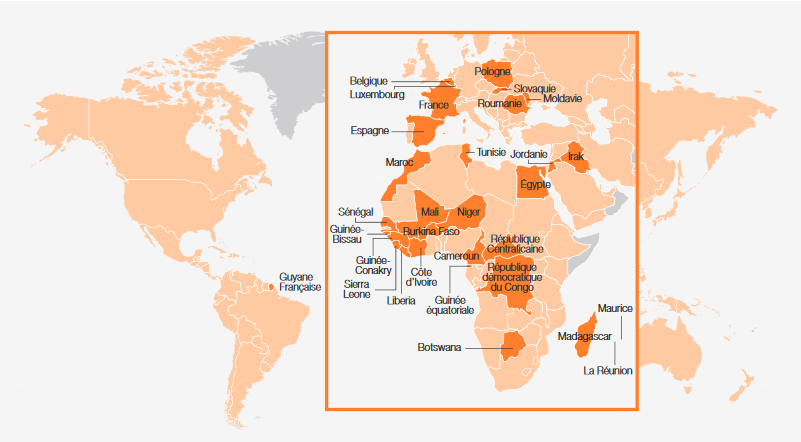
\includegraphics[scale=0.8]{./img/world_orange_2016.PNG}
    \caption{Carte des pays où est présent Orange en 2016}
\end{figure}
\paragraph*{}
Le groupe Orange est majoritairement présent en Europe et Afrique. Il est avant tout un leader de la téléphonie mobile avec un total de 202 millions de clients mobile en 2016 au niveau mondial. Orange est aussi leader dans le domaine de l’accès à Internet avec 18 millions de clients Internet haut débit fin 2016, 265 000 clients \gls{ftth} et 42 millions de clients sur la téléphonie fixe fin 2014 en France. Les pays où le groupe est le plus implanté sont la France, l’Espagne, la Pologne et la Roumanie. Depuis plusieurs années maintenant Orange essaie de se développer également en Afrique dans le domaine de la téléphonie mobile.
\paragraph*{}
Le secteur d’activité principal du groupe Orange reste les Télécommunications, en étant un opérateur téléphonique majeur en France et dans bien d’autres pays tels que la Pologne, l’Espagne, la Roumanie, Côte d’Ivoire, Égypte etc. Orange est également un fournisseur d’accès Internet et depuis quelques années élargit ses activités à la domotique, vente de contenus cinématographique et musical, médical, applications bancaires et automobiles etc.
\paragraph*{}
Les principaux concurrents d'Orange en France dans le domaine \gls{fai} sont principalement Free, Numéricâble, OVH, Nerim, Wifirst et Bouygues Télécoms. Et pour la téléphonie mobile ses principaux concurrents sont SFR, Free et Bouygues Télécom. Tandis qu'au niveau européen sur le domaine téléphonique et \gls{fai}, les principaux concurrents sont Deutsche Telekom, Vodafone et O2 en grande majorité.
\paragraph*{}
La branche où j’effectue mon alternance depuis 3 ans est \gls{ols}. Cette branche concerne tous ce qui touche à la recherche et au développement des produits Orange. Anciennement nommé France Télécom R\&D, puis \gls{olps} en 2007, et enfin rebaptisé \gls{ols} en 2017. Cette branche destinée à la recherche de l’ensemble du groupe Orange emploie 3500 personnes exclusivement en France. Fin 2012, le nombre de brevets déposés par Orange Labs s’élevaient à 7493. La R\&D est très importante pour Orange qui investit chaque année près de 900 millions d’euros dans ce secteur. \\

\subsection{Le contexte}
\subsubsection{Le Device Mangement à Orange}
\paragraph*{}
Mon alternance se déroule plus précisément au sein de l’équipe \gls{care}.  qui s’occupe de la gestion des équipements client, c’est-à-dire du « Device Management ».
\paragraph*{}
Le concept de « Device Management » possède plusieurs définitions selon les objets ou équipements gérés, et les équipes qui le mettent en place. Au sens de notre équipe, il est découpé en deux zones détaillées comme suis : 
\begin{itemize}
\subparagraph*{}
\item Le coté client, où l'on retrouve le réseau privé du client, dit le \gls{lan}, avec généralement divers équipements tels que, une passerelle Internet, un décodeur TV, un téléphone, une caméra \gls{ip}, des capteurs domotiques etc.
\item Le coté serveur, se trouvant chez Orange, où l'on va retrouver les serveurs, appelés \gls{acs} qui vont permettre de faire ce que l'on
nomme du Device Management.
\end{itemize}
\paragraph*{}
La communication entre un équipement et son \gls{acs} se fait via le protocole normalisé \gls{cwmp}. Ce protocole respecte le \gls{doctr069g} définie par le \gls{bbf}. Ainsi, chaque équipement et \gls{acs} doit respecter la norme décrite dans le \gls{doctr069g}. Il faut donc toujours veiller à ce que les équipements embarquent bien un client \gls{cwmp} respectant implémentant cette norme. Les \gls{acs}  doivent eux aussi rester à jour vis à vis de cette norme.
%Import Images
\begin{figure}[!ht]
    \center
    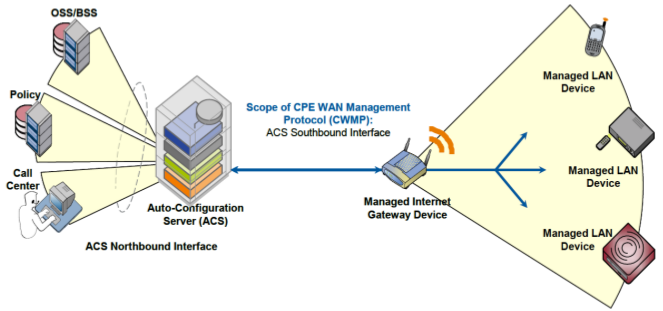
\includegraphics[scale=0.75]{./img/DM-TR-069-screen.png}
    \caption{Réseau de Device Management, côté \gls{acs} et côté Client}
\end{figure}
\paragraph*{}Le Device Management s'articule autour de quatre axes:
\begin{itemize}
\subparagraph*{}
\item Provsioning: Active ou désactive un service pour le client sur l'équipement adéquate; Applique le bon \gls{firmwareg} selon le service souscrit; Paramètre de manière personnalisé la configuration d'un équipement donné en fonction des service.
\item Assistance: Permet de diagnostiquer à distance un incident sur l'équipement; Déclencher à distance l'exécution d'action permettant de corriger un incident.
\item Tracking: Collecte et stocke des informations sur l'ensemble du parc client.
\item Maintenance: Permet la mise à jour de \gls{firmwareg} à différent temps souhaité.
\end{itemize}
\paragraph*{}
L’un des objectifs du Device Management, pour l’équipe \gls{care}, est d’apporter un service d’aide et de dépannage aux clients, tous en restant à distance. Dans le but de ne pas avoir à faire déplacer un technicien sur place, pour un problème qui peut être résolu à distance par l’exécution de scripts, lancement de test et analyse, correction de bug. Le rôle de l’équipe \gls{care}, est de concevoir l’intégration de ces outils qui pourront être utilisés à distance.
\paragraph*{}
La supervision et la maintenance du parc Orange sont d'autres activités dans le
périmètre de l'activité du Device Management. Ce parc contient les différents produits vendus par Orange et qu’Orange s'engage à maintenir. On comprend alors l'importance des activités de supervision et de maintenance. Pour gérer ce parc, Orange a besoin, entre autres, d'identifier les différents équipements présents et d'accéder à leurs  caractéristiques. Les outils de Device Management  développés au sein de l'équipe \gls{care} permettent, cette fois, de remonter aux \gls{acs} toutes les informations nécessaires pour superviser et maintenir le parc. Il permet également de mettre à jour et corriger des bugs en envoyant de nouvelles versions de \gls{firmwareg} aux équipements concernés. \\

\subsubsection{Document TR-069 et protocole normalisé CWMP}
\paragraph*{} Avant de continuer ce document, il est important d'apporter des précisions sur le \gls{doctr069g} et le protocole \gls{cwmp} qui en découle. 
\paragraph*{}Comme mentionné précédemment, le \gls{doctr069g} est le résultat d'un consortium de plusieurs industriels. Ce consortium, appelé le \gls{bbf}, ce compose de plus d'une centaine de membres dont Orange, CISCO, Deutch Telecom, Huawei, Juniper, le gouvernement du Canada, Intel et bien d'autre. Le \gls{bbf} vise à décrire la gestion des équipements clients, dit \gls{cpe}, par les serveurs de gestion d'équipements \gls{acs}. C'est par le \gls{doctr069g} que le \gls{bbf} décrit un standard permettant la communication entre \gls{cpe} et \gls{acs} pour une bonne gestion des équipements clients.
\paragraph*{} Ce standard décrit un modèle de donnée, que l'on nomme \gls{datamodelg}, comportant une partie commune, pour chaque équipement implémentant le \gls{doctr069g} et pouvant ainsi être manager par un \gls{acs}. Il décrit également différente méthode, que l'on nomme RPC Methode, obligatoire ou facultative, qui doivent être implémentées soit par l'ACS soit par le CPE. Parmi ces méthodes on peut cité les méthodes suivante:
\subparagraph*{}

\begin{table}
	\begin{tabularx}{17cm}{|l|X|l|}
		\hline
		RPC Method & Description & Implémenté par...\tabularnewline
		\hline
		Inform & Permet au CPE d'initier une session TR-069 & CPE\tabularnewline
		\hline
		InformResponse & Permet à l'ACS de répondre à un Inform. & ACS\tabularnewline
		\hline
		GetParameterValues & Permet de récupèrer la valeur d'un ou plusieurs 				paramètre du datamodel passé en paramètre. & ACS\tabularnewline
		\hline
		GetParameterValuesResponse & Permet au CPE de répondre à un 						GetParameterValues en indiquant la/les valeur(s) du/des paramètre(s) 				demandé(s) par l'ACS & CPE\tabularnewline
		\hline
		SetParameterValues & Permet de modifier la valeur d'un ou plusieurs 				paramètre du datamodèle passé en paramètre. & ACS\tabularnewline
		\hline
		SetParameterValuesResponse & Permet au CPE de répondre à un 						SetParameterValues en indiquant si la demande a pu être réaliser. & CPE\tabularnewline
		\hline
	\end{tabularx}
	\centering
	\caption{Liste des RPC méthodes rencontrées dans ce document.}
\end{table}
\paragraph*{} Plus précisément, un \gls{cpe}, afin de pouvoir échanger avec un \gls{acs} doit implémenter le \gls{doctr069g} sous la forme du protocole \gls{cwmp}. Ce protocole est transporté par du \gls{http} et encapsulé dans des messages SOAP. La création de session TR-069 ce fait toujours par le CPE. L'ACS ne peut pas créer de session, en revanche il peut demander au CPE qu'il vienne créer une session sur demande, en lui envoyant un \gls{http} GET à une URL exposé par le CPE, avec les bons identifiants. 

\subsection{Objectifs envisagés}
\subsubsection{Première année}
\subsubsection{Deuxième année}
\subsubsection{Troisième année}

\newpage
\section{Monté en compétence sur le protocole CWMP}
\subsection{Création d'un ACS Servlet}
\subsection{Études d'équipements}
\subsubsection{Présentation du réseau isolé}
\subsubsection{Test DNS}
\subsubsection{Test de comportement TR-069 d'équipement}
\subsection{Étude de client CWMP}
\subsubsection{Client EasyCWMP}
\subsubsection{Client tr69agent d'Orange}
\subsubsection{Résultats} %conséquence : création du toolkit !
\subsection{Impact sur mon parcours}

\newpage
\section{Projet principal: Conception et développement d'un outil de test}
\subsection{Contexte}
\subsection{Présentation}
\subsection{Méthode de projet}
\subsection{Travail de préparation}
\subsubsection{Recherche de solution technique}
\subsubsection{Analyse de faisabilité}
\subsection{Conception}
\subsection{Réalisation}
\subsubsection{Travail en équipe}
\subsubsection{Développement}
\subsection{Déploiement}
\subsubsection{Environement}
\subsection{Communication et utilisateur}
\subsection{Livrable du projet}
\subsection{Difficultés, solutions et compétences acquises}
\subsection{Bilan et apport personnel du projet}

\newpage
\section{Transfert de compétences}

\newpage
\section{Bilan de compétences}

\newpage
\section{Conclusion}
\subsection{Atteintes des objectifs}
\subsection{Progression}
\subsection{Synthèse de parcours}

\end{document}
